%!TEX root = ./template-skripsi.tex
%-------------------------------------------------------------------------------
%                            BAB II
%               TINJAUAN PUSTAKA DAN DASAR TEORI
%-------------------------------------------------------------------------------

\chapter{TINJAUAN PUSTAKA DAN DASAR TEORI}                


\section{Landasan Teori}

  \subsection{SCARA}
  \begin{figure}[H]
  	\centering
  	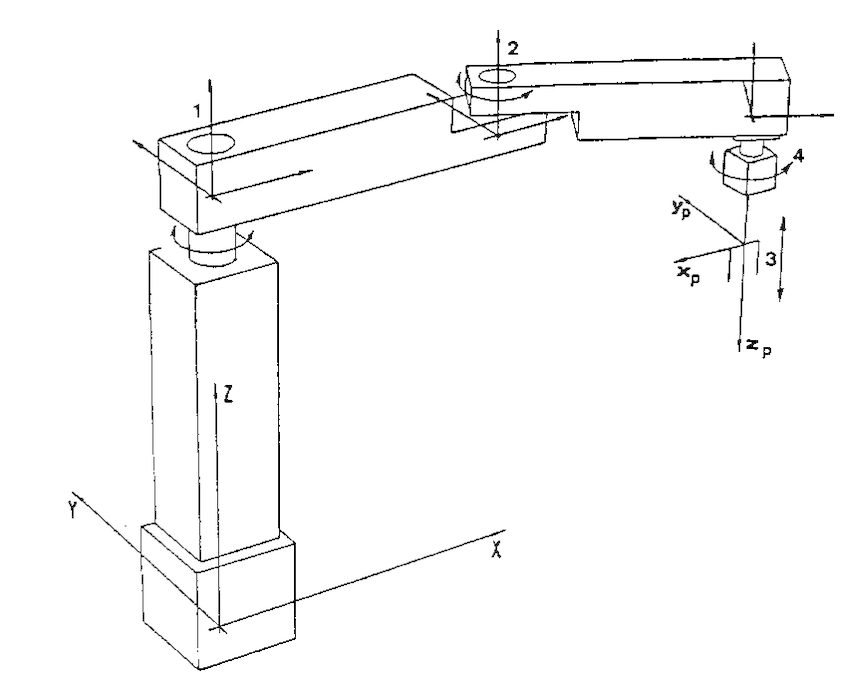
\includegraphics[width=4.33cm]{scara.png}
  	\caption{Pergerakan Robot SCARA}
  \end{figure}
  
  SCARA merupakan singkatan dari \emph{Selective Compliant Assembly Robot Arm}. Robot ini pertama kali dibuat oleh perusahaan USA bernama Adept pada 1984 dan diklasifikasikan sebagai robot industri. Sistem penggerak robot SCARA merupakan pergerakan langsung pada lengan tanpa bantuan sistem \emph{belt} keculai pada bagian \emph wirst, sehingga membuat mekanisme gerakannya bekerja cepat, sederhana namun tetap akurat. Robot ini banyak digunakan sebagai robot \emph {aseembly part} dengan ukuran yang kecil degan kecepatan sedang. 
  
  Robot SCARA yang digunakan pada penelitian ini menggunakan robot SCARA dengan nama Serpent-2. Robot Serpent-2 memiliki dua \textit{horizontal joint} yaitu bagian \textit{shoulder, elbow}dan \textit{wrist} yang dikendalikan oleh motor servo. Sedangkan pada bagian \textit{vertical joint} yang berfungsi sebagai naik turun dan buka tutup dari \emph wirst, dikendalikan oleh pneumatik yang dikontrol oleh \emph {valve relay}. Sehingga, gerakan yang terdapat pada robot SCARA dapat diklasifikasikan sebagai gerakan mengambil dan menempatkan objek. 
  \begin{table}[H]
  	\centering
  	\caption{Spesifikasi Robot Serpent-2}
  	\resizebox{6cm}{!}{%
  		\begin{tabular}{|l|l|}
  			\hline
  			Main arm length      & 360 mm$$\hspace{2cm} 		\\ \hline
  			Fore arm length      & 290 mm$$  				\\ \hline
  			Shoulder movement    & 180 °$$  		\\ \hline
  			Elbow movement       & 200 °$$   		\\ \hline
  			Wrist rotation       & 360 °$$ 		\\ \hline
  			Up \& down movement  & 150 mm$$   				\\ \hline
  			Maximum tip velocity & 3.0 kg$$  				\\ \hline

  		\end{tabular}%
  	}
  \end{table}

 Pada bagian motor servo, robot serpent-2 menggunakan tiga buah sensor \emph feedback yang berguna sebagai pemberi nilai posisi pada masing-masing motor servo. Sensor \emph feedback yang digunakan pada robot SCARA ini menggunakan potensiometer yang memberikan nilai analog dan kemudian diproses oleh Arduino Mega 2560. Nilai ini, nantinya untuk memproses gerak kinematika dari robot SCARA tersebut sesuai dengan posisi yang diinginkan.
 \begin{table}[H]
 	\centering
 \caption{Spesifikasi Motor DC pada robot Serpent-2}
 \resizebox{11cm}{!}{%
 	\begin{tabular}{|l|l|}
 		\hline
 		Moments of inertia of the main arm ($J_{1}$)    							& $$ 				\\ \hline
 		Moments of inertia of the fore arm ($J_{2}$)    							& $$ 				\\ \hline
 		Masses of the main arm	($m_{1}$)											& $$   					\\ \hline
 		Masses of the fore arm  ($m_{2}$)     										& $$   					\\ \hline
 		Motor and equivalent inertias ($J_{m}$)      								& $$ 			\\ \hline
 		Back emf constants for main arm and fore arm motor ($K_{e1}=K_{e2}$)  		& $$   				\\ \hline
 		Armature resistance for main arm and fore arm motor($R_{a1}=R_{a2}$)		& $$  					\\ \hline
 		Armatures inductances for main and fore arm motor  ($L_{a1}=L_{a2}$) 		& $$ 						\\ \hline
 	\end{tabular}%
 }
\end{table}


  \subsection{Kinematika Robot}
  Kinematika robot adalah studi analisis
  pergerakan kaki atau lengan robot terhadap
  sistem kerangka koordinat acuan yang diam
  atau bergerak tanpa memperhatikan gaya yang
  menyebabkan pergerakan tersebut. Model
  kinematika merepresentasikan hubungan \emph{end
  effector} dalam ruang tiga dimensi dengan
  variabel sendi dalam ruang sendi.
  
  Dalam kinematika dikenal istilah \emph{forward}
  kinematika dan \emph{invers} kinematika. \emph{Forward}
  kinematika adalah metode untuk menentukan
  orientasi dan posisi \emph{end effector} dari besarnya
  sudut sendi dan panjang link kaki robot.
  Sedangkan \emph{invers} kinematika merupakan
  kebalikan dari forward kinematika yaitu metode
  untuk mengetahui nilai sudut pada sendi-sendi
  yang diperlukan agar end effector dapat
  mencapai posisi yang dikehendaki. 
  
   \subsection{Arduino Mega 2560}
   \begin{figure}[H]
   	\centering
   	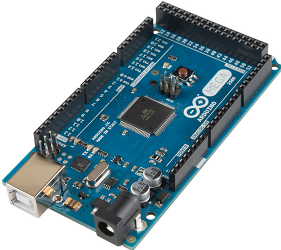
\includegraphics[width=4.33cm]{gambar/arduino_mega.png}
   	\caption{ Arduino Mega 2560}
   \end{figure}
   
  Board Arduino Mega 2560 adalah sebuah Board Arduino yang menggunakan IC Mikrokontroler ATmega 2560.Board ini memiliki Pin I/O yang relatif banyak, 54 digital Input / Output,15 buah di antaranya dapat digunakan sebagai output PWM, 16 buah analog Input, 4 UART. Arduino Mega 2560 di lengkapi cristal 16. Mhz 
  	
  
   \subsection{Processing IDE}
  \begin{figure}[H]
  	\centering
  	
\includegraphics[width=4.33cm]{logo_processing.png}
  	\caption{Processing IDE}
  \end{figure}
  \emph{Processing} adalah lingkungan pemrograman sederhana yang dibuat untuk  memudahkan pengembangkan aplikasi yang berorientasi visual dengan penekanan pada animasi dan menyediakan respon balik yang instan kepada pengguna melalui interaksi didalamnnya. Para pengembang menginginkan cara untuk "membuat sketsa" ide dalam kode. Karena kemampuannya telah berkembang selama dekade terakhir, \emph{Processing} telah digunakan untuk pekerjaan tingkat produksi yang lebih maju. Awalnya dibangun sebagai ekstensi khusus domain ke Java yang ditargetkan untuk seniman dan desainer, Processing telah berevolusi menjadi desain penuh dan alat \emph{prototyping} yang digunakan untuk pekerjaan instalasi skala besar, gambar gerak, dan visualisasi data yang kompleks.
   

  
  

% Baris ini digunakan untuk membantu dalam melakukan sitasi
% Karena diapit dengan comment, maka baris ini akan diabaikan
% oleh compiler LaTeX.
\begin{comment}
\bibliography{daftar-pustaka}
\end{comment}
